\documentclass[10pt,a4paper]{article}

\usepackage[T1]{fontenc}
\usepackage[utf8]{inputenc}
\usepackage{lmodern}
\usepackage[margin=1.62cm]{geometry}
\usepackage{setspace}
\usepackage{amsmath,amssymb,mathtools}
\usepackage{booktabs}
\usepackage{tikz}
\usetikzlibrary{arrows.meta,positioning}
\usepackage{enumitem}
\usepackage{caption}
\usepackage{hyperref}
\hypersetup{colorlinks=true,linkcolor=black,citecolor=black,urlcolor=blue}

\setstretch{1.04}
\setlength{\parskip}{0.32em}
\setlength{\parindent}{1.05em}
\setlist{nosep,leftmargin=1.2em}

\newcommand{\cmax}{C_{\max}}

\title{\large Research for Solving Multi-Target Scheduling of School Bag Factory Production by Using Resource-Coupled Heterogeneous Graph Attention}
\author{Computer Science Short Paper\\Companion to the system-design thesis}
\date{October 2026}

\begin{document}
\maketitle
\vspace{-1.6em}

\begin{abstract}
\noindent
A school-bag line is a flexible job shop in which an operation starts only when a machine, a skilled operator, and often a shared die or thread lot are free together. The same decision must serve several targets: makespan, tardiness, energy, and workload balance. This paper presents resource-coupled heterogeneous graph attention (RCH-GAT). Each feasible action is a bundle, and each bundle is scored by one-hop attention over an operation node, a machine node, an operator node, and a shop node that reads token contention. A preference vector opens the nodes, so one score can be asked to protect due dates or energy. Twenty coefficients are identified by the cross-entropy method on a school-bag simulator. On twenty nominal order books the score, without maintenance, finishes in \(1234\) minutes and \(211\,\mathrm{kWh}\), against about \(1521\) minutes and \(303\,\mathrm{kWh}\) for first-in-first-out. Colour features are specified and, under ample lots, nearly silent. The numbers are estimates of this implementation.
\end{abstract}

\section{Introduction}

Classical dispatching chooses the next job by a single key. First-in-first-out uses release time. Shortest processing time uses duration. Earliest due date uses the promise date. Apparent tardiness cost mixes slack and duration with a look-ahead \cite{vepsalainen1987}. Each rule is rational for the target written into its key, and each is silent about the targets that are not. A school-bag shift cares about all of them at once. Cutting, embroidery, lockstitch, bartack, hardware, inspection, and packing can run on more than one resource, but the resource is not a machine alone. An operator without the skill, or a khaki thread lot already held by another body, makes the machine idle in the schedule even while the machine record says it is free.

Graph methods already represent flexible job shops. The disjunctive graph separates conjunctive precedence from machine choices \cite{roy1964,adams1988}. Heterogeneous graph networks learn embeddings of operations and machines and pick an operation--machine pair by reinforcement learning \cite{song2023,park2021,zhang2020}. Those models are the right lineage. Textile shops have been searched with ant-colony methods \cite{chen2024}, and energy together with labour has been treated as a many-objective flexible job shop \cite{gong2019}. They still stop one resource short of this factory. The pair \((operation, machine)\) does not name the operator, and it does not name the die or the colour lot. A policy trained on that pair can recommend a bundle the shop cannot start.

The contribution of this paper is a score that refuses that recommendation before it is ranked. The action is the bundle
\begin{equation}
a = (O_{ij},\, k,\, o,\, q),
\label{eq:bundle}
\end{equation}
where \(O_{ij}\) is operation \(i\) of order \(j\), \(k\) is a machine, \(o\) is an operator, and \(q\) is the token the step requires, or a null token when the step needs none. Infeasible bundles are masked. Feasible bundles are compared by preference-conditioned attention on a four-node graph. The executable policy is one hop and is identified by cross-entropy search. A multi-layer heterogeneous graph attention network, trained by proximal policy optimisation \cite{velickovic2018,schulman2017}, is the same idea at a larger data scale. It is specified and not the source of the tables below.

\section{Shop, targets, and the masked bundle}

Orders follow one of three routes: backpack (eight operations), trolley (seven), or sports sack (six). Nine machines sit in seven groups. Eight operators cover them, with a skill matrix that is mostly sparse. Two cutting dies are shared. Thread lots have capacities: navy, black, red, and grey allow two concurrent users, and khaki allows one. A shortage scenario drops navy, red, and khaki to one.

Processing time depends on quantity, size, machine speed, operator skill, and machine health \(h_k\),
\begin{equation}
p_{ijko}(h_k) = \tau_{ij}\,\frac{q_j}{80}\,\zeta_j\,\frac{1 + 0.85\, h_k^{1.15}}{v_k\,\sigma_{ok}} .
\label{eq:ptime}
\end{equation}
At \(h_k = 0\) this is an ordinary flexible-job-shop time. On the worn automatic cutter used in the worked example, \(h = 0.58\) and the health factor is about \(1.45\).

The four targets reported with the schedule are makespan \(\cmax = \max_j C_j\), total tardiness \(T = \sum_j \max(0, C_j - d_j)\), energy \(E\) in kilowatt-hours, and workload imbalance \(B\), the standard deviation of busy minutes. Expected failures \(\Phi\) are carried as a fifth term inside the scalar used for identification,
\begin{equation}
J_\omega = \omega_1 \frac{\cmax}{\cmax^{\mathrm{FIFO}}} + \omega_2 \frac{T}{T^{\mathrm{FIFO}}} + \omega_3 \frac{E}{E^{\mathrm{FIFO}}} + \omega_4 \frac{B}{B^{\mathrm{FIFO}}} + 0.12\,\frac{\Phi}{\Phi^{\mathrm{FIFO}}} .
\label{eq:scalar}
\end{equation}
The balanced preference used for identification is \(\omega = (0.34, 0.33, 0.18, 0.15)\). Dividing by the first-in-first-out value on the same book keeps a long tardiness number from drowning a makespan ratio.

A candidate enters the feasible set \(\mathcal{F}(t)\) only when the operation's predecessor is finished, the order has been released, the machine and the operator are free, the operator's skill on that machine group is positive, and the required token has residual capacity. The mask is the feasibility proof. The score never repairs an illegal assignment after the fact, because an illegal assignment is never scored.

\section{One-hop heterogeneous attention}

Each candidate induces four nodes. The operation node carries time, setup, slack, and remaining critical work. The machine node carries health, load imbalance, cycle energy, and failure probability. The operator node carries the skill gap. The shop node carries how many ready operations want the same colour, the same die pool, or the same machine group. Figure~\ref{fig:graph} is one candidate. The shop graph at time \(t\) is the union of these graphs over \(\mathcal{F}(t)\). Attention does not mix two candidates before their scores are compared.

\begin{figure}[ht]
\centering
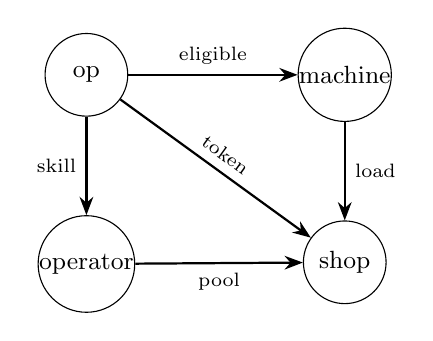
\begin{tikzpicture}[
  n/.style={draw, circle, minimum size=1.05cm, inner sep=0pt, font=\small, align=center},
  arr/.style={-{Stealth}, thick}
]
\node[n] (op) {op};
\node[n, right=2.15cm of op] (m) {machine};
\node[n, below=1.25cm of op] (o) {operator};
\node[n, below=1.25cm of m] (s) {shop};
\draw[arr] (op) -- node[above, font=\scriptsize] {eligible} (m);
\draw[arr] (op) -- node[left, font=\scriptsize] {skill} (o);
\draw[arr] (m) -- node[right, font=\scriptsize] {load} (s);
\draw[arr] (o) -- node[below, font=\scriptsize] {pool} (s);
\draw[arr] (op) -- node[above, font=\scriptsize, sloped] {token} (s);
\end{tikzpicture}
\caption{One candidate bundle. Precedence is already enforced by the ready set, so it is not an edge inside the candidate.}
\label{fig:graph}
\end{figure}

Twelve raw costs are scaled near the unit interval: processing time over \(45\), setup over \(11\), negative slack over \(180\), a critical-ratio term, health, excess load over \(80\), cycle energy, failure probability, colour contention, die contention, group contention, and the skill gap below \(1.05\). Positive weights \(w\), obtained by exponentiating stored logarithms, form four node costs \(c_u\). Four keys \(\kappa_u\) are fixed groupings of the same raw costs and are used only to place attention. The preference opens the nodes,
\begin{align}
\pi_{\mathrm{op}} &= 0.55 + g_1(\omega_1+\omega_2), &
\pi_{\mathrm{m}} &= 0.55 + g_2(\omega_3+0.5\omega_1), \nonumber\\
\pi_{\mathrm{o}} &= 0.45 + g_3\omega_4, &
\pi_{\mathrm{s}} &= 0.45 + g_4(\omega_2+0.25).
\label{eq:open}
\end{align}
Time and due date open the operation node. Energy, and part of makespan, open the machine node, because a worn cutter destroys both. Balance opens the operator node. Due date also opens the shop node, because a free machine with a seized lot is how a promise is missed. Attention is a softmax of bias plus opened key,
\begin{equation}
\alpha_u = \frac{\exp(a_u + \pi_u \kappa_u)}{\sum_{u'} \exp(a_{u'} + \pi_{u'} \kappa_{u'})},
\qquad
\psi(a) = \sum_u \alpha_u \, \pi_u \, c_u .
\label{eq:psi}
\end{equation}
The dispatcher takes \(\arg\min_{a \in \mathcal{F}(t)} \psi(a)\).

The identified weights, in the order of the twelve raw costs, are
\begin{align*}
w = (&0.288,\ 1.029,\ 0.731,\ 0.235,\ 0.606,\ 5.660,\\
&0.912,\ 1.269,\ 0.133,\ 0.917,\ 0.353,\ 1.657).
\end{align*}
Load, skill, failure, and setup dominate. The colour weight is \(0.133\). Attention biases on the four nodes are \(1.082\), \(0.969\), \(-0.707\), and \(0.672\). The gates are \(1.023\), \(0.852\), \(1.892\), and \(-1.621\). At the balanced preference the shop-node opening is negative, about \(-0.49\), and in the cutter example below the shop node receives about three percent of the attention. Token pressure is present in the graph and nearly inactive in this fit. That is an outcome of identification, not a missing feature.

On a navy shell of quantity \(80\), size M, base time \(24\) minutes, and no setup, Cutter-A (\(v=1.28\), \(h=0.58\)) takes \(27.3\) minutes and Cutter-B (\(v=0.74\), \(h=0.22\)) takes \(37.3\) minutes. Shortest processing time selects A. The score gives \(\psi(A) = 2.108\) and \(\psi(B) = 0.776\), and selects B, because health, failure, and power on A outweigh the shorter cycle. This comparison does not yet insert maintenance. Maintenance is the companion technology of the thesis and is turned off in the RCH column of the estimate.

\section{Identification and estimate}

The twenty coefficients were identified by the cross-entropy method: population \(36\), elite \(8\), \(28\) generations, starting from a log-prior that already blends processing time, slack, and health. The training books are seeds \(11\), \(23\), \(37\), and \(41\). The best scalar relative to first-in-first-out fell from about \(0.450\) to \(0.366\). Changing \(\omega\) in \eqref{eq:open} without repeating the search does not trace a reliable Pareto front. A new preference is a new identification.

Table~\ref{tab:nominal} reports means over twenty paired books, seeds \(1000\)--\(1019\), sixteen orders, nominal wear and nominal token capacities. RCH is the graph score with maintenance off. The other rows are rules that share the same mask and the same plant. Tardiness standard deviations are several hundred minutes, so a gap of a few tens of minutes in tardiness is not a ranking. Makespan and energy gaps are large beside their spreads.

\begin{table}[ht]
\centering
\caption{Nominal books. Times are minutes. Energy is kilowatt-hours. RCH is the graph score without maintenance.}
\label{tab:nominal}
\small
\begin{tabular}{lrrrrr}
\toprule
Method & Makespan & Tardiness & On time & Energy & Failures \\
\midrule
FIFO & 1520.7 & 2761.4 & 0.519 & 303.2 & 18.02 \\
SPT & 1547.6 & 512.8 & 0.816 & 268.3 & 15.56 \\
EDD & 1545.4 & 212.1 & 0.891 & 299.3 & 16.95 \\
ATC & 1631.8 & 274.7 & 0.863 & 299.1 & 17.44 \\
RCH & 1234.4 & 260.9 & 0.853 & 211.0 & 10.13 \\
\bottomrule
\end{tabular}
\end{table}

Against first-in-first-out, RCH shortens the day by about \(286\) minutes and cuts energy from \(303\) to \(211\,\mathrm{kWh}\). Against the best classical energy, shortest processing time at \(268\,\mathrm{kWh}\), the saving is about \(57\,\mathrm{kWh}\). Imbalance falls from about \(370\) to \(260\) busy-minute standard deviation. Expected failures fall from the mid-teens to about \(10\), which is the part of failure avoidance that a health-aware score can buy without being allowed to renew a machine. Tardiness, \(261\) minutes, sits with earliest due date's \(212\) inside a spread of hundreds of minutes. The due-date claim on an ordinary day is that the score does no clear harm.

Under a rush of four orders released at minute \(220\), RCH finishes in \(1676\) minutes at \(302\,\mathrm{kWh}\) with \(17.9\) expected failures, against about \(2000\) minutes, \(408\,\mathrm{kWh}\), and \(27\) failures for earliest due date. Under thread shortage the same score finishes in \(1225\) minutes and \(208\,\mathrm{kWh}\). Zeroing the three contention features moves the shortage makespan of the full system, which includes maintenance, from \(1039\) to \(1075\) minutes. The shift has the correct sign and is small beside a \(90\)-minute spread. Resource coupling is a real correction when lots are tight. It is not the source of the large makespan and energy gaps, which remain when those features are removed.

\section{What the fit is doing}

The cross-entropy search did not spread weight evenly. Table~\ref{tab:w} keeps the costs whose weights exceed \(0.9\), which are the ones that move \(\psi\) on a typical candidate. Load imbalance is an order of magnitude above processing time. A machine that is already busy is expensive even when its cycle is short. Skill sits next, so a slow substitute operator is not a free way to grab an idle machine. Failure and setup outrank the raw minutes of the cycle. Colour, at \(0.133\), does not appear in the table because it lost the identification.

\begin{table}[ht]
\centering
\caption{Dominant positive weights after identification. Smaller weights (processing time \(0.288\), critical ratio \(0.235\), colour \(0.133\), group \(0.353\), health \(0.606\), slack \(0.731\)) remain in the score.}
\label{tab:w}
\small
\begin{tabular}{llr}
\toprule
Cost & Node & Weight \\
\midrule
Load imbalance & machine & 5.660 \\
Skill gap & operator & 1.657 \\
Failure probability & machine & 1.269 \\
Sequence setup & operation & 1.029 \\
Die contention & shop & 0.917 \\
Cycle energy & machine & 0.912 \\
\bottomrule
\end{tabular}
\end{table}

Dispatch is then a short loop. At the current time, list every operation whose predecessor is done and whose order is released. For each such operation, list eligible free machines, skilled free operators, and a free token if the step needs one. Score each surviving bundle by \eqref{eq:psi} and commit the minimum. Advance the clock to the next instant at which a machine and an operator are both free, release tokens of finished work, and repeat. No priority list is frozen at the start of the shift. A rush order enters the list at its release minute and is scored with whatever health the machines have by then.

That loop is why RCH still helps when maintenance is absent. On the rush books it finishes in \(1676\) minutes and \(302\,\mathrm{kWh}\) with \(17.9\) expected failures, against about \(2000\) minutes, \(408\,\mathrm{kWh}\), and \(27\) failures for earliest due date. On the accelerated-wear books it finishes in \(1782\) minutes and \(310\,\mathrm{kWh}\) with \(30.6\) expected failures, against about \(2059\) minutes, \(384\,\mathrm{kWh}\), and \(39\) failures. Preferring the healthy manual cutter, a less loaded lockstitch, and a sufficiently skilled operator is the whole of this gain. Renewal of a worn tool is a further gain, and it belongs to the companion paper. Changing the preference without repeating the search is not a substitute for either.

\section{Conclusion}

RCH-GAT makes the school-bag decision a masked bundle and scores that bundle by preference-conditioned attention on operation, machine, operator, and shop nodes. On the simulator the identified one-hop score shortens and cools the day relative to first-in-first-out, shortest processing time, earliest due date, and apparent tardiness cost, and it keeps tardiness inside the band of the due-date rules. The colour weight learned on these books is small, which matches a small shortage ablation. A deeper graph network remains the scalable form of the same score. It was not the policy that produced Table~\ref{tab:nominal}.

\begin{thebibliography}{99}
\bibitem{garey1976} M.~R. Garey, D.~S. Johnson, and R.~Sethi. The complexity of flowshop and jobshop scheduling. \emph{Mathematics of Operations Research}, 1(2):117--129, 1976.
\bibitem{roy1964} B.~Roy and B.~Sussmann. Les probl\`emes d'ordonnancement avec contraintes disjonctives. Note DS no.~9 bis, SEMA, 1964.
\bibitem{adams1988} J.~Adams, E.~Balas, and D.~Zawack. The shifting bottleneck procedure for job shop scheduling. \emph{Management Science}, 34(3):391--401, 1988.
\bibitem{brandimarte1993} P.~Brandimarte. Routing and scheduling in a flexible job shop by tabu search. \emph{Annals of Operations Research}, 41:157--183, 1993.
\bibitem{pinedo2016} M.~L. Pinedo. \emph{Scheduling: Theory, Algorithms, and Systems}. Springer, 5th edition, 2016.
\bibitem{vepsalainen1987} A.~P.~J. Vepsalainen and T.~E. Morton. Priority rules for job shops with weighted tardiness costs. \emph{Management Science}, 33(8):1035--1047, 1987.
\bibitem{gong2019} X.~Gong, T.~De~Pessemier, L.~Martens, and W.~Joseph. Energy- and labor-aware flexible job shop scheduling under dynamic electricity pricing: A many-objective optimization investigation. \emph{Journal of Cleaner Production}, 209:1077--1094, 2019.
\bibitem{vaswani2017} A.~Vaswani et al. Attention is all you need. In \emph{Advances in Neural Information Processing Systems}, 2017.
\bibitem{velickovic2018} P.~Veli{\v c}kovi{\'c} et al. Graph attention networks. In \emph{International Conference on Learning Representations}, 2018.
\bibitem{kool2019} W.~Kool, H.~van Hoof, and M.~Welling. Attention, learn to solve routing problems! In \emph{International Conference on Learning Representations}, 2019.
\bibitem{zhang2020} C.~Zhang, W.~Song, Z.~Cao, J.~Zhang, P.~S. Tan, and X.~Chi. Learning to dispatch for job shop scheduling via deep reinforcement learning. In \emph{Advances in Neural Information Processing Systems}, 2020.
\bibitem{park2021} J.~Park, J.~Chun, S.~H. Kim, Y.~Kim, and J.~Park. Learning to schedule job-shop problems: representation and policy learning using graph neural network and reinforcement learning. \emph{International Journal of Production Research}, 59(11):3360--3377, 2021.
\bibitem{song2023} W.~Song, X.~Chen, Q.~Li, and Z.~Cao. Flexible job-shop scheduling via graph neural network and deep reinforcement learning. \emph{IEEE Transactions on Industrial Informatics}, 19(2):1600--1610, 2023.
\bibitem{schulman2017} J.~Schulman, F.~Wolski, P.~Dhariwal, A.~Radford, and O.~Klimov. Proximal policy optimization algorithms. arXiv:1707.06347, 2017.
\bibitem{chen2024} F.~Chen, W.~Xie, J.~Ma, J.~Chen, and X.~Wang. Textile flexible job-shop scheduling based on a modified ant colony optimization algorithm. \emph{Applied Sciences}, 14(10):4082, 2024.
\end{thebibliography}

\end{document}
